\chapter{k-Means Clustering}
\label{ch:kmeans-clustering}

\newthought{Hierarchical clustering is not suitable for larger data sets} due to the prohibitive size of the distance matrix: with 30 thousand objects, the distance matrix already has almost one billion elements. An alternative approach that avoids using the distance matrix is k-means clustering.

K-means clustering randomly selects k centers (with k specified in advance). Then it alternates between two steps. In one step, it assigns each point to its closest center, thus forming k clusters. In the other, it recomputes the centers of the clusters. Repeating these two steps typically convergences quite fast; even for the big data sets with millions of data points it usually takes just a couple of tens or hundreds iterations.

Orange's add-on Educational provides a widget Interactive k-means, which illustrates the algorithm.

Use the Paint widget to paint some data - maybe five groups of points. Feed it to Interactive k-means and set the number of centroids to 5. You may get something like this.

\marginnote{Try rerunning the clustering from new random positions and observe how the centers conquer the territory. Exciting, isn't it?}

\begin{figure}[h]
    \centering
    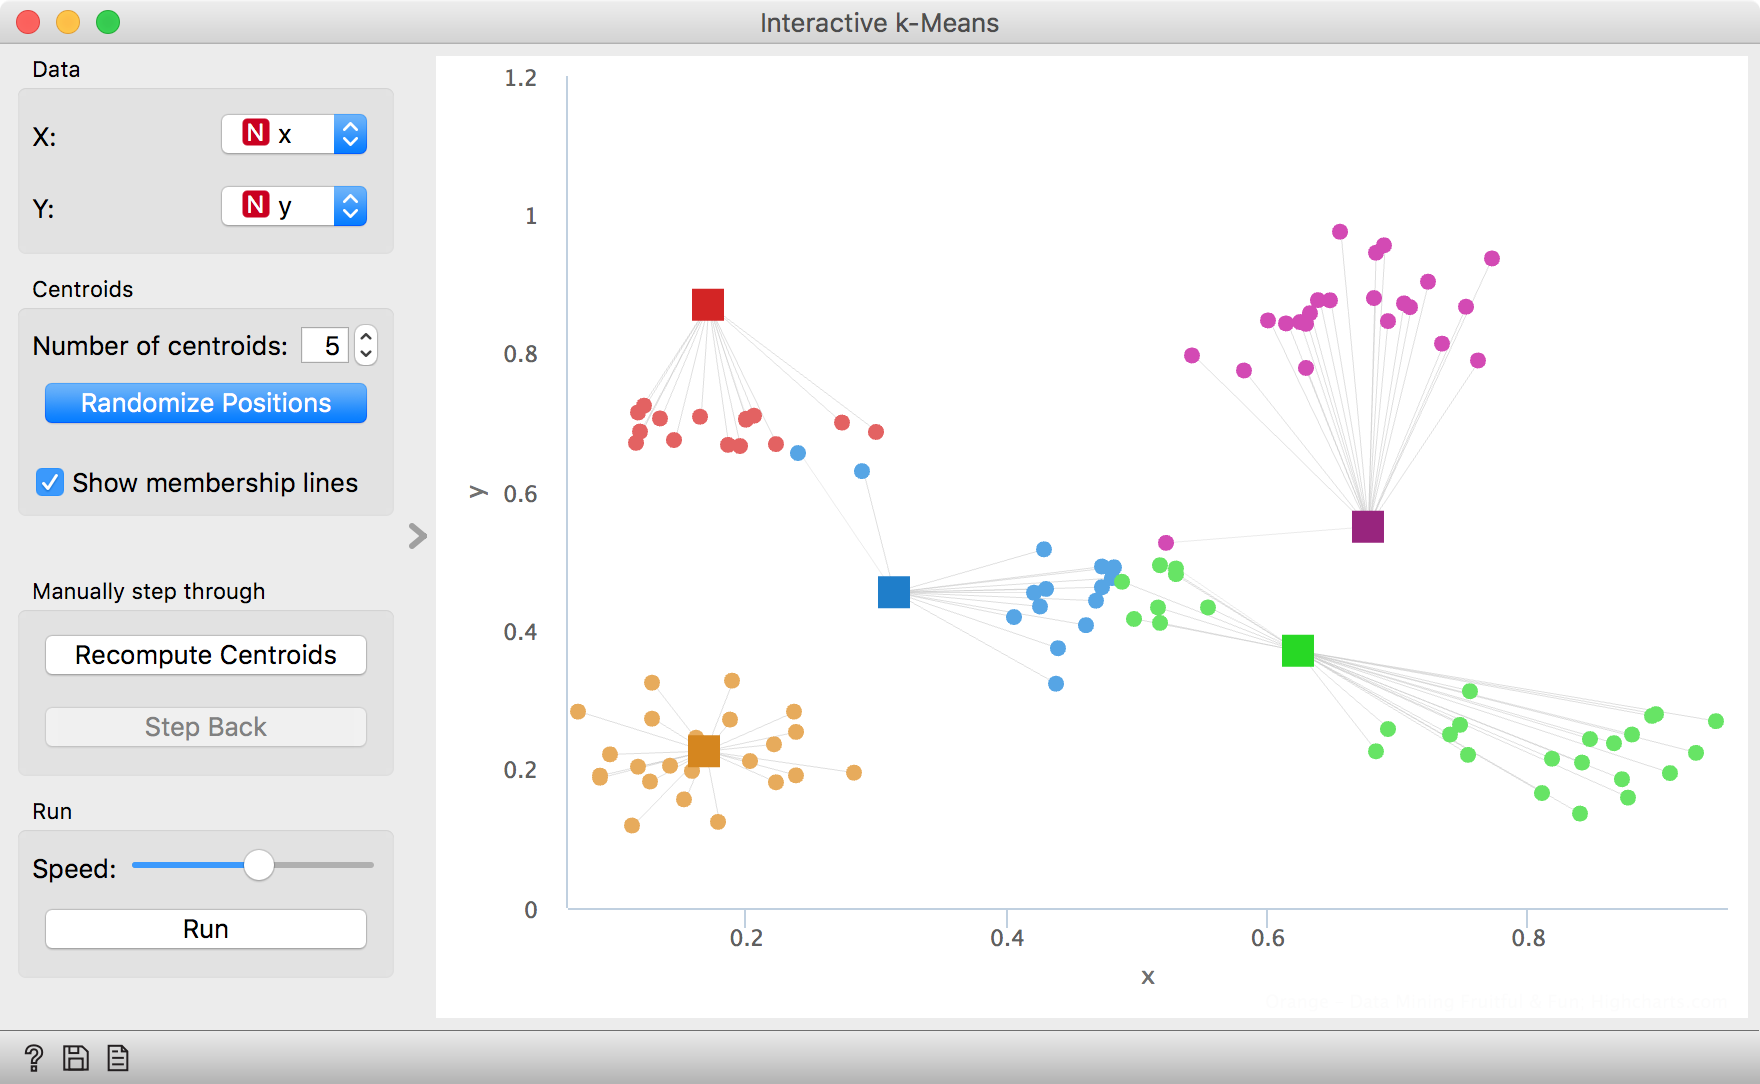
\includegraphics[width=\linewidth]{interactive-kmeans.png}
    \caption{$\;$} % empty caption for proper pagesetting
\end{figure}

Keep pressing Recompute Centroids and Reassign Membership until it stops changes. With this simple, two-dimensional data it will take just a few iterations; with more points and features, it can take longer, but the principle is the same.

How do we set the initial number of clusters? That's simple: we choose the number that gives the optimal clustering.

Well then, how do we define the optimal clustering? This one is a bit harder. We want small distances between points in the same cluster and large distances between points from different clusters. Pick one point, and let A be its average distance to the data points in the same cluster and let B represent the average distance to the points from the closest other cluster. (The closest cluster? Just compute B for all other clusters and take the lowest value.) The value (B - A) / max(A, B) is called silhouette; the higher the silhouette, the better the point fits into its cluster. The average silhouette across all points is the silhouette of the clustering. The higher the silhouette, the better the clustering.

Now that we can assess the quality of clustering, we can run k-means with different values of parameter k (number of clusters) and select k which gives the largest silhouette.

For this, we abandon our educational toy and connect Paint to the widget k-Means. We tell it to find the optimal number of clusters between 2 and 8, as scored by the Silhouette.

\begin{figure}[h]
    \centering
    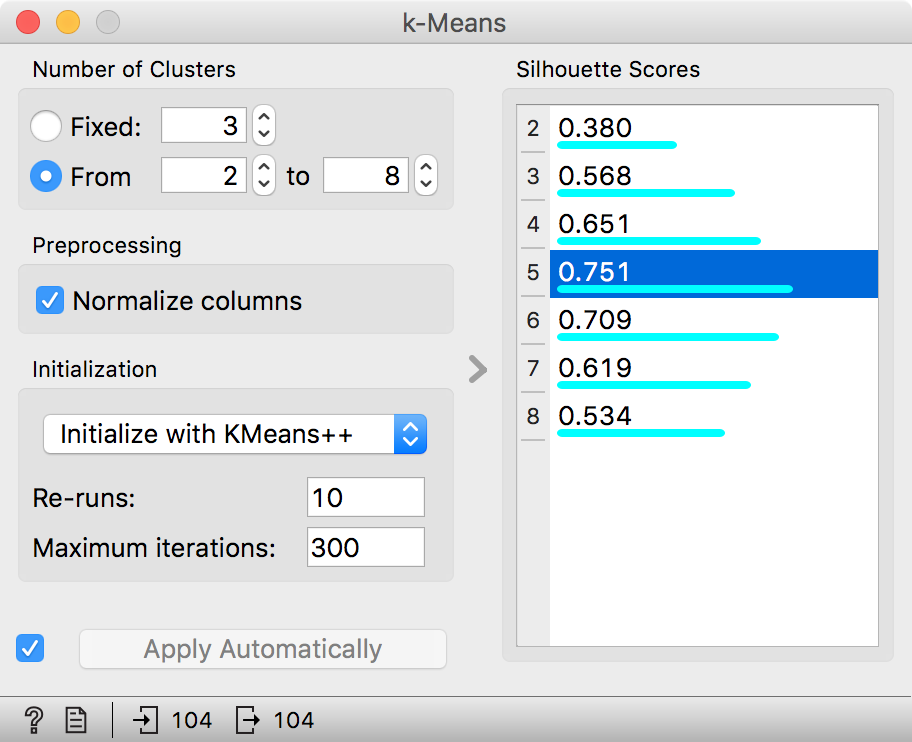
\includegraphics[width=\linewidth]{kmeans-silhouette.png}
    \caption{$\;$} % empty caption for proper pagesetting
\end{figure}

\newpage

Works like charm.

Except that it often doesn't. First, the result of k-means clustering depends on the initial selection of centers. With unfortunate selection, it may get stuck in a local optimum. We solve this by re-running the clustering multiple times from random positions and using the best result. Second, the silhouette sometimes fails to correctly evaluate the clustering. Nobody's perfect.

Time to experiment. Connect the Scatter Plot to k-Means. Change the number of clusters. See if the clusters make sense. Could you paint the data where k-Means fails? Or where it really works well?

\begin{figure}[h]
    \centering
    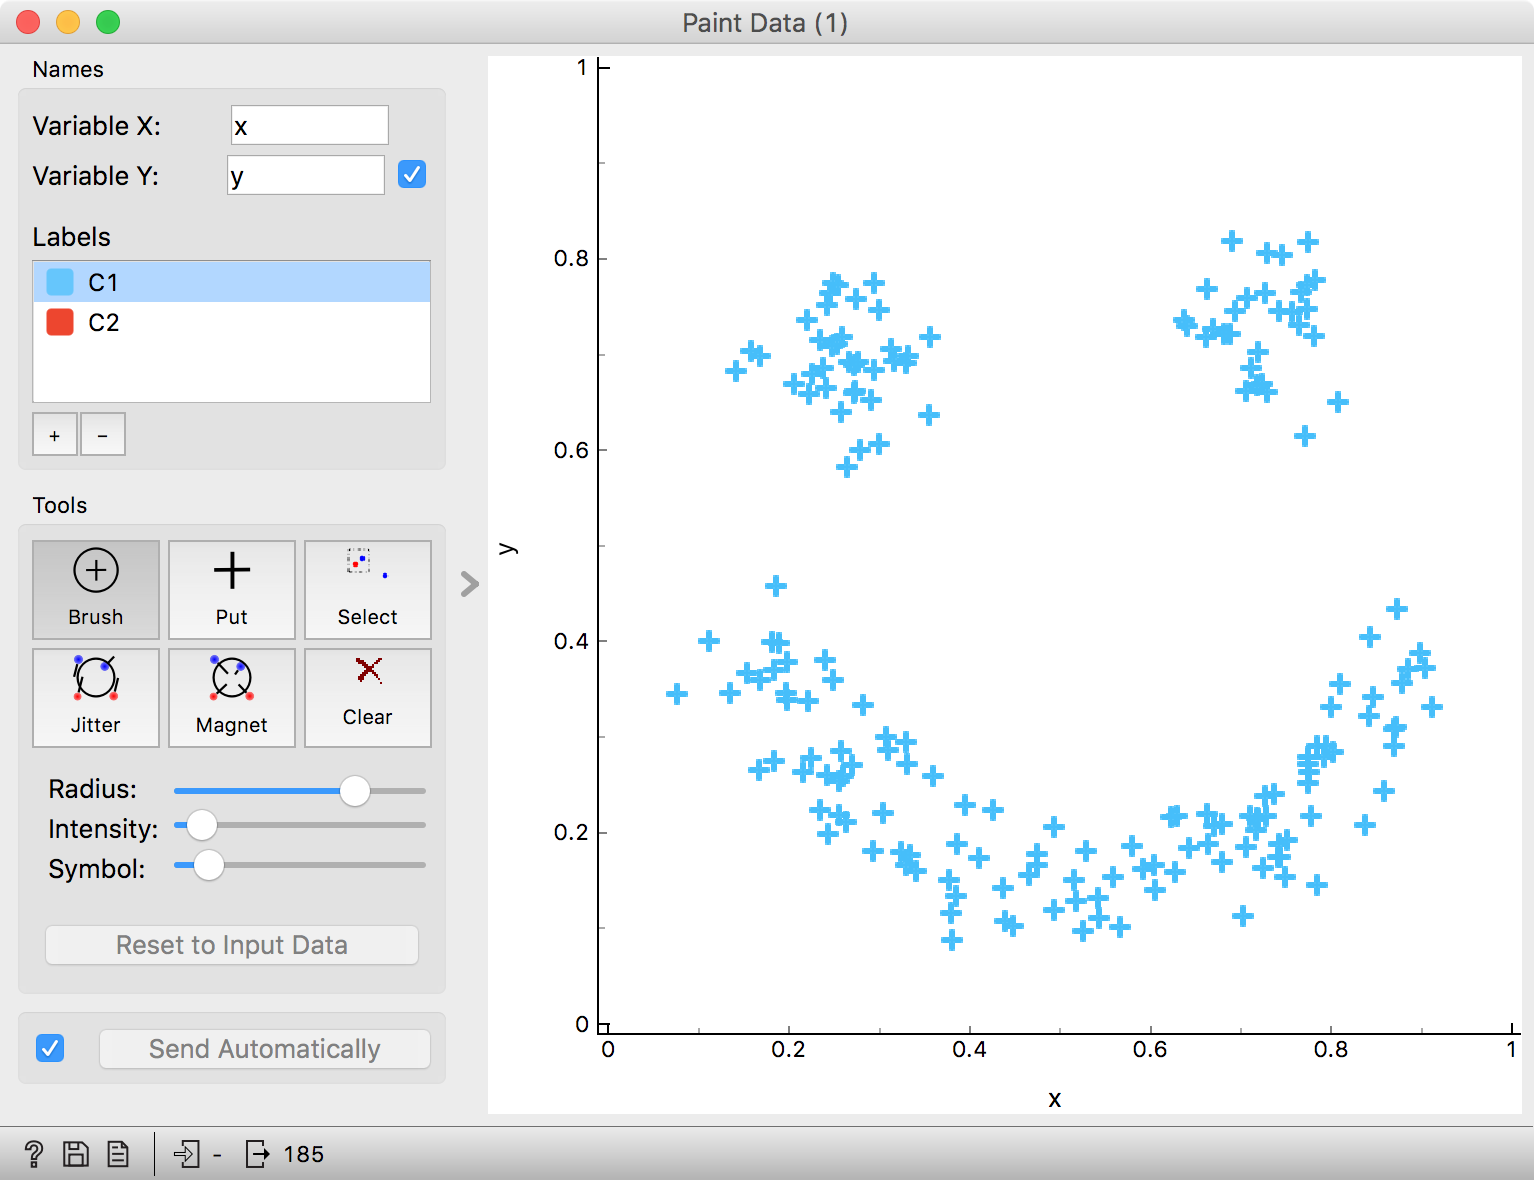
\includegraphics[width=\linewidth]{smiley-face.png}
    \caption{$\;$} % empty caption for proper pagesetting
\end{figure}
